\documentclass[tikz,border=2pt]{standalone}
\usepackage[T1]{fontenc}
\usepackage{lmodern}
\usetikzlibrary{arrows.meta,positioning}

\definecolor{ink}{HTML}{253247}
\definecolor{muted}{HTML}{657286}
\definecolor{grid}{HTML}{D7DDE7}
\definecolor{panel}{HTML}{F7F9FC}
\definecolor{blue}{HTML}{3478BF}
\definecolor{teal}{HTML}{2A9D8F}
\definecolor{orange}{HTML}{F29E4C}
\definecolor{red}{HTML}{D65A4A}
\definecolor{purple}{HTML}{7B61A8}

\begin{document}
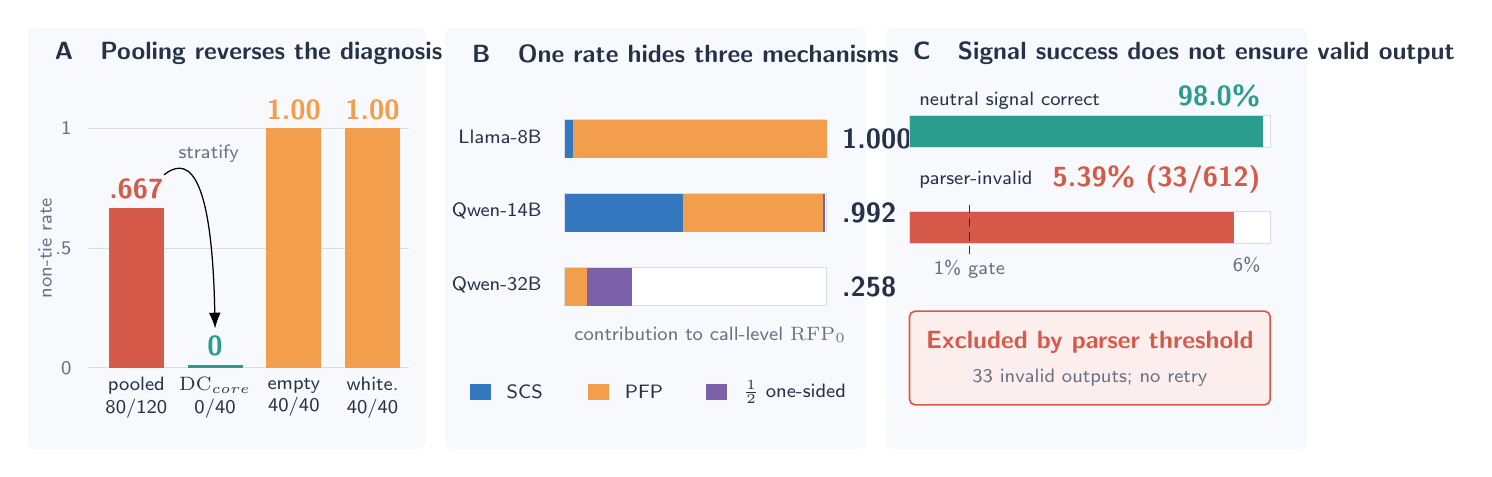
\begin{tikzpicture}[x=1cm,y=1cm,font=\sffamily\scriptsize,text=ink]
  % Panel backgrounds.
  \fill[panel,rounded corners=2pt] (0,0) rectangle (5.05,5.35);
  \fill[panel,rounded corners=2pt] (5.30,0) rectangle (10.65,5.35);
  \fill[panel,rounded corners=2pt] (10.90,0) rectangle (16.25,5.35);

  % Panel A: pooled value versus null strata.
  \node[anchor=west,font=\sffamily\bfseries\small] at (0.22,5.02) {A\quad Pooling reverses the diagnosis};
  \draw[grid] (0.76,1.03) -- (4.84,1.03);
  \draw[grid] (0.76,2.55) -- (4.84,2.55);
  \draw[grid] (0.76,4.07) -- (4.84,4.07);
  \node[anchor=east,text=muted] at (0.68,1.03) {0};
  \node[anchor=east,text=muted] at (0.68,2.55) {.5};
  \node[anchor=east,text=muted] at (0.68,4.07) {1};
  \node[rotate=90,text=muted] at (0.22,2.55) {non-tie rate};
  \fill[red] (1.03,1.03) rectangle (1.73,3.06);
  \fill[teal] (2.03,1.03) rectangle (2.73,1.07);
  \fill[orange] (3.03,1.03) rectangle (3.73,4.07);
  \fill[orange] (4.03,1.03) rectangle (4.73,4.07);
  \node[font=\sffamily\bfseries,text=red] at (1.38,3.30) {.667};
  \node[font=\sffamily\bfseries,text=teal] at (2.38,1.31) {0};
  \node[font=\sffamily\bfseries,text=orange] at (3.38,4.31) {1.00};
  \node[font=\sffamily\bfseries,text=orange] at (4.38,4.31) {1.00};
  \node[align=center] at (1.38,0.65) {pooled\\80/120};
  \node[align=center] at (2.38,0.65) {$\mathrm{DC}_{core}$\\0/40};
  \node[align=center] at (3.38,0.65) {empty\\40/40};
  \node[align=center] at (4.38,0.65) {white.\\40/40};
  \draw[-{Latex[length=2mm]},line width=.45pt,text=muted] (1.73,3.48) .. controls (1.98,3.68) and (2.34,3.68) .. (2.38,1.53);
  \node[fill=panel,inner sep=1pt,text=muted] at (2.30,3.75) {stratify};

  % Panel B: canonical decomposition of same-quality false preference.
  \node[anchor=west,font=\sffamily\bfseries\small] at (5.52,5.02) {B\quad One rate hides three mechanisms};
  \node[anchor=east] at (6.65,3.96) {Llama-8B};
  \node[anchor=east] at (6.65,3.02) {Qwen-14B};
  \node[anchor=east] at (6.65,2.08) {Qwen-32B};
  \foreach \y in {3.70,2.76,1.82} {
    \fill[white] (6.82,\y) rectangle (10.15,\y+0.48);
    \draw[grid] (6.82,\y) rectangle (10.15,\y+0.48);
  }
  % widths use a 3.33 cm unit scale.
  \fill[blue]   (6.82,3.70) rectangle (6.93,4.18);
  \fill[orange] (6.93,3.70) rectangle (10.15,4.18);
  \fill[blue]   (6.82,2.76) rectangle (8.32,3.24);
  \fill[orange] (8.32,2.76) rectangle (10.10,3.24);
  \fill[purple] (10.10,2.76) rectangle (10.13,3.24);
  \fill[orange] (6.82,1.82) rectangle (7.10,2.30);
  \fill[purple] (7.10,1.82) rectangle (7.68,2.30);
  \node[anchor=west,font=\sffamily\bfseries] at (10.22,3.94) {1.000};
  \node[anchor=west,font=\sffamily\bfseries] at (10.22,3.00) {.992};
  \node[anchor=west,font=\sffamily\bfseries] at (10.22,2.06) {.258};
  \node[anchor=west,text=muted] at (6.82,1.45) {contribution to call-level $\mathrm{RFP}_0$};
  \fill[blue] (5.62,0.62) rectangle (5.88,0.82);
  \node[anchor=west] at (5.96,0.72) {SCS};
  \fill[orange] (7.12,0.62) rectangle (7.38,0.82);
  \node[anchor=west] at (7.46,0.72) {PFP};
  \fill[purple] (8.62,0.62) rectangle (8.88,0.82);
  \node[anchor=west] at (8.96,0.72) {$\frac12$ one-sided};

  % Panel C: the parser gate overrides an attractive signal score.
  \node[anchor=west,font=\sffamily\bfseries\small] at (11.12,5.02) {C\quad Signal success does not ensure valid output};
  \node[anchor=west] at (11.20,4.42) {neutral signal correct};
  \fill[white] (11.20,3.83) rectangle (15.78,4.23);
  \draw[grid] (11.20,3.83) rectangle (15.78,4.23);
  \fill[teal] (11.20,3.83) rectangle (15.69,4.23);
  \node[anchor=east,font=\sffamily\bfseries,text=teal] at (15.78,4.48) {98.0\%};
  \node[anchor=west] at (11.20,3.42) {parser-invalid};
  \fill[white] (11.20,2.61) rectangle (15.78,3.01);
  \draw[grid] (11.20,2.61) rectangle (15.78,3.01);
  \fill[red] (11.20,2.61) rectangle (15.32,3.01);
  \draw[ink,densely dashed,line width=.55pt] (11.96,2.47) -- (11.96,3.13);
  \node[anchor=north,text=muted] at (11.96,2.53) {1\% gate};
  \node[anchor=east,font=\sffamily\bfseries,text=red] at (15.78,3.42) {5.39\% (33/612)};
  \node[anchor=east,text=muted] at (15.78,2.34) {6\%};
  \fill[red!10,rounded corners=2pt] (11.20,0.56) rectangle (15.78,1.75);
  \draw[red,rounded corners=2pt,line width=.6pt] (11.20,0.56) rectangle (15.78,1.75);
  \node[font=\sffamily\bfseries\small,text=red] at (13.49,1.36) {Excluded by parser threshold};
  \node[text=muted] at (13.49,0.91) {33 invalid outputs; no retry};
\end{tikzpicture}
\end{document}
